\documentclass[conference]{IEEEtran}
\usepackage{cite}
\usepackage{amsmath,amssymb,amsfonts}
\usepackage{algorithmic}
\usepackage{graphicx}
\usepackage{textcomp}
\usepackage{xcolor}
\usepackage{pgfplots}
\pgfplotsset{compat=1.18}

\usepackage{tikz}
\usetikzlibrary{arrows.meta, positioning, shapes.geometric}

\begin{document}

\title{The Calçotada Protocol: \ Equity Peg Tokens for Decentralized Venture Capital}

\author{\IEEEauthorblockN{Author Name}
\IEEEauthorblockA{\textit{Organization} \\
City, Country \\
email@example.com}}

\maketitle

\begin{abstract}
This paper introduces the Calçotada Protocol, a blockchain-based approach designed to democratize access to early-stage venture capital by issuing tokenized convertible notes pegged directly to startup valuations. By addressing the inherent inequities and innovation limitations of traditional venture capital models, our protocol provides liquidity and governance rights through decentralized autonomous organizations (DAOs), bridging the gap between non-crypto startups and blockchain funding mechanisms.
\end{abstract}

\begin{IEEEkeywords}
Blockchain, Venture Capital, Decentralized Finance, Tokenization, Equity Peg Token, DAO
\end{IEEEkeywords}

\section{Introduction: Unlocking Foundational Capital for Everyone}

Venture capital (VC) acts simultaneously as the engine and gatekeeper of innovation, deciding which startups receive funding and consequently determining who shapes the products and services of tomorrow. This concentration of influence leads to what Acemoglu and Johnson describe as a "tunnel vision" in their seminal work \textit{Power and Progress} (2023), wherein the future is shaped not by societal necessities or disruptive innovations, but by trends favored by large capital holders. This cycle perpetuates itself: venture capital firms backed by substantial resources dictate innovation agendas, consolidating wealth and reinforcing their dominance over technological and economic progress.

This entrenched model of early-stage investing not only restricts innovation to predefined agendas but exacerbates inequality by excluding smaller investors from the highest-return investment opportunities—namely, seed-stage equity rounds. Consequently, retail investors resort to speculative assets such as memecoins, seeking the kinds of outsized returns historically realized in early-stage VC funding, but without genuine exposure to underlying innovation or governance rights.

Blockchain technology offers a foundational shift in this dynamic by enabling decentralized autonomous organizations (DAOs) and token-based governance models to democratize access to venture-stage capital and decision-making processes.

The Calçotada Protocol is our practical response to this systemic imbalance. It provides a structured, transparent on-chain mechanism that directly links token ownership to startup valuations and governance rights. Through tokenized convertible notes, the protocol allows individual investors—not just large institutions—to meaningfully participate in both the financial and governance aspects of promising startups at their earliest stages.

This protocol was specifically developed to meet the funding requirements of The Calçotada Company, a food-tech startup with a disruptive and validated business model. The innovative nature of this company has inspired the development of Equity Peg Tokens as a foundational mechanism for exploring Decentralized Autonomous Venture Capital (DAVC). Moreover, the protocol aims explicitly to bridge the gap between traditional, non-crypto startups and blockchain-based funding mechanisms, thus enabling broader, more inclusive access to early-stage venture capital opportunities.

\section{Prior Art and Related Work}

Blockchain technology has significantly altered the landscape of startup financing, leading to an emergence of novel funding mechanisms primarily through Initial Coin Offerings (ICOs) and token sales. Guangye Cao (2023), in his seminal paper \textit{``Startup Financing: Token vs Equity"}, highlights that blockchain-based startups commonly prefer token issuance over traditional equity due to enhanced liquidity and lower return expectations from investors, driven by early liquidity rather than intrinsic valuation \cite{cao2023token}. However, this financing model predominantly targets crypto-native startups building decentralized applications (dApps) or blockchain protocols. Thus, these tokens typically derive value from speculative market dynamics rather than a measurable relationship to company success or valuation milestones \cite{howell2020initial, catalini2019some}.

Several foundational studies underline these market dynamics. Howell et al. (2020) find that token success in ICOs correlates closely with disclosure practices and speculative expectations rather than fundamental valuation metrics tied explicitly to a startup’s success \cite{howell2020initial}. Similarly, Chod and Lyandres (2021) point out that token financing frequently introduces agency problems, as entrepreneurs are incentivized to underproduce since their revenues are not strictly pegged to token values or vice versa \cite{chod2021theory}. Cong et al. (2021) also note the prevalence of speculative pricing, driven largely by investor expectations about future platform popularity rather than underlying business fundamentals \cite{cong2021tokenomics}.

The literature further emphasizes a structural shortcoming in current token funding models, specifically their inherent inability to effectively bridge token valuation to real-world company performance and equity milestones. For example, the widely-used Simple Agreement for Future Tokens (SAFT), while attempting to integrate traditional funding elements, still ultimately relies on future speculative market conditions rather than measurable startup outcomes \cite{mendelson2019saft}. Meanwhile, token-warrant structures and automated convertible notes introduced by ConsenSys and others attempt to blend equity and token economics but do not provide explicit pegging mechanisms between token value and company valuation, leaving substantial room for market speculation and volatility \cite{lw2019token}.

In this context, token financing as historically implemented has primarily appealed to blockchain-focused ventures, offering limited utility to traditional non-crypto enterprises seeking structured and valuation-based early-stage financing mechanisms. Despite clear liquidity advantages outlined by Cao (2023) and others, the absence of a stable and measurable peg to equity valuation remains a critical gap in current blockchain funding structures.

Addressing precisely this gap, the Calçotada Protocol proposes an innovative framework: a \textit{Tokenized Convertible Note (TCN)} explicitly pegged to company valuation. By bridging traditional valuation-linked financial instruments with blockchain-enabled liquidity, the protocol uniquely positions itself as a solution capable of transcending speculative market dynamics and offering structured equity participation and governance rights to retail investors.

\section{Extended Analysis of Dual-Token Models}

\subsection{Dual-Asset Token Models}

A growing class of decentralized finance and DAO systems use a dual-token model, combining:

\begin{itemize}
    \item A non-fungible or governance token for voting/access
    \item A fungible token for utility or financial participation
\end{itemize}

Examples include:

\textbf{Charged Particles} offers a framework allowing NFTs to hold fungible tokens—creating hybrid assets, but not necessarily valuation‑pegged economic instruments~\cite{chargedparticles2022}.

\textbf{Tensor DAO} issues a governance token (TNSR) alongside protocol usage tokens—holders vote and receive revenue-share—but tokens are not directly pegged to outside company valuations~\cite{tensor2025}.

\textbf{Origyn Protocol} uses OGY as a fungible utility/governance token alongside provenance NFTs—though again, without a peg to company performance~\cite{origyn2022}.

Academic work on NFT authentication and hybrid structures exists (e.g. Talgar \& Banach~\cite{talgar2024dao}, Avrilionis \& Hardjono~\cite{avrilionis2022assetproxy}), but these focus on access control or metadata consistency—not on funding mechanics or value-redemption.

\subsection{Research Gap}

While dual-token models are gaining traction in DeFi and NFT ecosystems, none explicitly link the fungible token’s value to company performance or guarantee redemption pegged to valuation. Existing models focus on speculative pricing, membership perks, or governance, not on treating tokens as digital equity with built-in mechanisms to ensure economic alignment.

\subsection{Contribution of the Calçotada Protocol}

The Calçotada Protocol bridges these gaps by:

\begin{itemize}
    \item Issuing \textbf{Founder NFTs} for governance and access;
    \item Issuing \textbf{RMSC fungible tokens} with a strict, externally validated PEG to company valuation;
    \item Enforcing buyback commitments on-chain via transparent smart contracts and external oracles;
    \item Combining liquidity, governance, and valuation parity in a single dual-token financial architecture.
\end{itemize}



\section{Fundamental Key Assets and On-Chain Accountancy}
A primary innovation of the Calçotada Protocol is the incorporation of on-chain accountancy as a transparent foundation for venture valuations, investor returns, and protocol trust. This section reviews the strategic assets necessary for protocol integrity and public confidence, highlighting how on-chain financial tracking directly informs estimated valuations and buyback commitments.

\subsection{On-Chain Accountancy}
Unlike traditional venture frameworks—where assessment of company value and investor ROI rely on opaque, often delayed financial reporting—the Calçotada Protocol mandates continuous, verifiable financial accounting on-chain. All critical financial flows (revenue, costs, operational reserves, distributions) are recorded in transparent smart contracts.

This enables:
\begin{itemize}
    \item \textbf{Real-time, tamper-proof valuation:} Investors and protocol governors can view up-to-date figures at any point, reducing ambiguity or information asymmetry.
    \item \textbf{Reliable ROI estimates:} Using industry-standard financial metrics (see next subsection), the protocol can project and periodically update company valuations and potential ROI for token holders.
    \item \textbf{Algorithmic buyback triggers:} Token buyback amounts and conditions are derived from on-chain accounting data, automating investor returns and aligning incentives.
\end{itemize}

\subsection{Valuation Methodology and Financial Modeling}
To ensure that buybacks reflect fundamentally justified valuations, the protocol leverages conventional startup valuation techniques. The accompanying \texttt{Tokenomics RMSC.ods} model calculates buyback scenarios and expected valuations based on revenue multiples, discounted cash flows, or other startup-typical factors. These methods are encoded in oracles or contract formulas, supporting automated, auditable financial flows without need for off-chain negotiations.

This structure allows retail and institutional investors to benefit from return estimates and exit strategies anchored in both blockchain transparency and accepted financial practice—even before actual company liquidity events.

\subsection{Additional Key Assets}
\begin{itemize}
    \item \textbf{Smart Contracts:} All protocol commitments (NFTs, RMSC tokenomics, buybacks, treasury reserve) are transparently on-chain.
    \item \textbf{External Oracles:} For validation of off-chain revenue or event triggers as needed.
    \item \textbf{Decentralized Governance:} Founder NFTs enable participatory protocol upgrades and control structures.
\end{itemize}

\section{Protocol Architecture}

\usetikzlibrary{arrows.meta, positioning, shapes.geometric}

\begin{figure}[ht]
\centering
\scalebox{0.5}{%
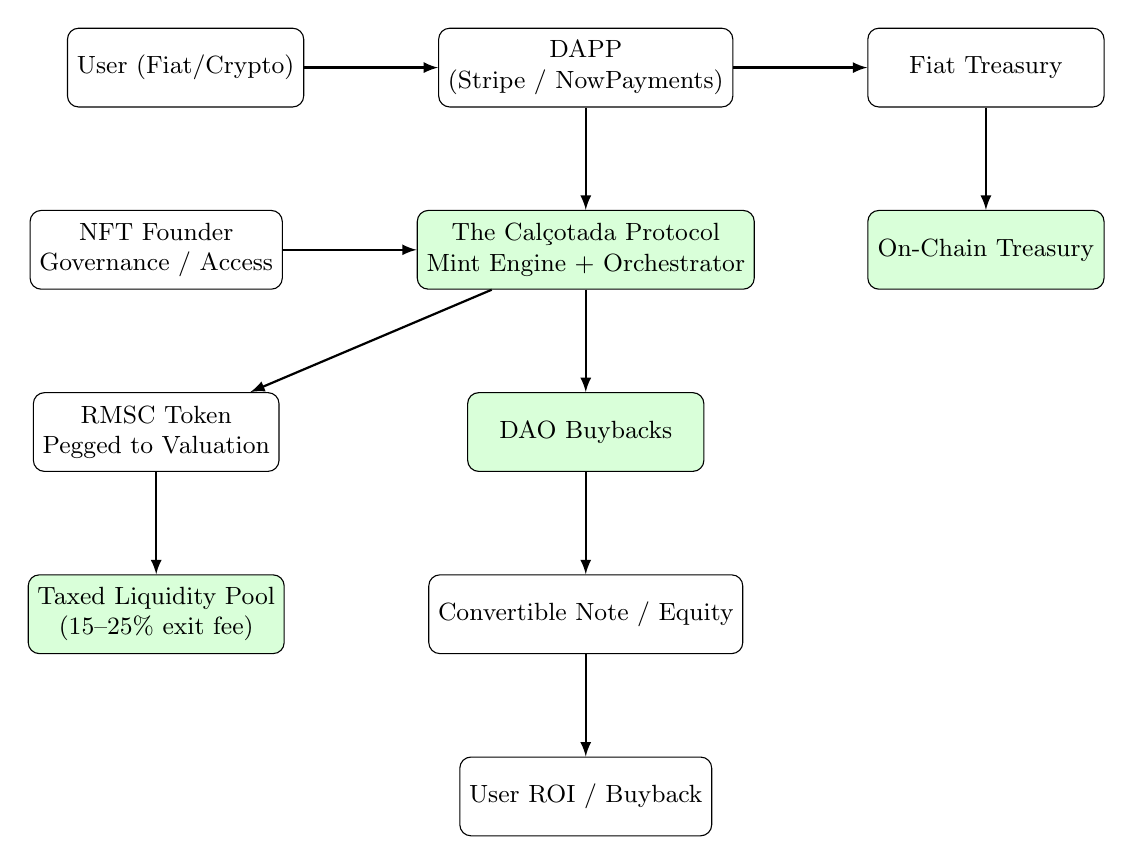
\begin{tikzpicture}[node distance=1.3cm and 1.7cm, every node/.style={font=\small}]

% Styles
\tikzstyle{box} = [draw, rounded corners, align=center, minimum width=3cm, minimum height=1cm, fill=white]
\tikzstyle{greenbox} = [box, fill=green!15]
\tikzstyle{arrow} = [->, thick, >=latex]

% Nodes
\node[box] (user) {User (Fiat/Crypto)};
\node[box, right=of user] (dapp) {DAPP\\(Stripe / NowPayments)};
\node[box, right=of dapp] (fiat) {Fiat Treasury};
\node[greenbox, below=of fiat] (onchain) {On-Chain Treasury};

\node[greenbox, below=of dapp] (protocol) {The Calçotada Protocol\\Mint Engine + Orchestrator};

\node[box, left=of protocol] (nft) {NFT Founder\\Governance / Access};
\node[box, below=of nft] (rmsc) {RMSC Token\\Pegged to Valuation};

\node[greenbox, below=of protocol] (dao) {DAO Buybacks};
\node[box, below=of dao] (equity) {Convertible Note / Equity};
\node[box, below=of equity] (payback) {User ROI / Buyback};

\node[greenbox, below=of rmsc] (tlp) {Taxed Liquidity Pool\\(15–25\% exit fee)};

% Arrows
\draw[arrow] (user) -- (dapp);
\draw[arrow] (dapp) -- (fiat);
\draw[arrow] (fiat) -- (onchain);
\draw[arrow] (dapp) -- (protocol);

\draw[arrow] (nft) -- (protocol);
\draw[arrow] (protocol) -- (rmsc);
\draw[arrow] (protocol) -- (dao);
\draw[arrow] (dao) -- (equity);
\draw[arrow] (equity) -- (payback);
\draw[arrow] (rmsc) -- (tlp);

\end{tikzpicture}%
}%
\caption{Simplified architecture of the Calçotada Protocol: dual-token issuance and treasury-integrated valuation peg.}
\end{figure}

% 
\usepackage{tikz-uml}

\begin{figure}[ht]
\centering
\scalebox{0.5}{%
\begin{tikzpicture}[node distance=1.6cm and 1.8cm]

% LEFT COLUMN
\node (rmsc) [tokencontract] {RMSCToken \nodepart{second} ERC20 \\ Peg Mechanism \nodepart{third} mint() \\ burn() \\ buyback()};
\node (nft) [tokencontract, below=of rmsc] {FounderNFT \nodepart{second} ERC721 \\ Governance \nodepart{third} vote() \\ access()};

% CENTER
\node (protocol) [orchestrator, right=of rmsc, yshift=-1cm] {THE CALÇOTADA \nodepart{second} Orchestrator \\ Mint Engine \nodepart{third} Controller Functions};

% RIGHT
\node (fiatinput) [treasurycontract, above=of protocol] {FiatInputContract \nodepart{second} Deposit \nodepart{third} Withdraw};
\node (onchain) [treasurycontract, below=0.8cm of fiatinput] {OnChainTreasury \nodepart{second} Store \nodepart{third} Audit};
\node (paytreasury) [treasurycontract, right=of fiatinput] {PaydayTreasury \nodepart{second} Pay \nodepart{third} Distribute};

\node (daobuybacks) [contract, right=of protocol, yshift=-1cm] {DAOBuybacks \nodepart{second} Convertible Note \\ SAFE + Equity \nodepart{third} execute() \\ validate()};
\node (daotube) [contract, right=of daobuybacks] {DAOTube \nodepart{second} Buyback Handler \nodepart{third} process() \\ distribute()};
\node (instruments) [contract, below=of daotube] {Instruments \nodepart{second} Financial Tools \nodepart{third} convert() \\ redeem()};
\node (userwallet) [contract, below=of instruments] {UserWallet \nodepart{second} Balance Manager \nodepart{third} deposit() \\ withdraw()};

% BOTTOM
\node (taxpool1) [treasurycontract, below=of nft, xshift=3cm] {TaxedLiquidityPool \nodepart{second} Exit Tax Handler \nodepart{third} collect() \\ redistribute()};
\node (taxpool2) [treasurycontract, below=of daobuybacks] {TaxedLiquidityPool \nodepart{second} Exit Tax Handler \nodepart{third} collect() \\ redistribute()};

% ARROWS
\draw [arrow] (fiatinput) -- (onchain);
\draw [arrow] (fiatinput) -- (paytreasury);
\draw [arrow] (paytreasury) |- (daotube);
\draw [arrow] (onchain) -- (protocol);

\draw [arrow] (rmsc) -- (protocol);
\draw [arrow] (nft) -- (protocol);

\draw [arrow] (protocol) -- (daobuybacks);
\draw [arrow] (daobuybacks) -- (daotube);
\draw [arrow] (daotube) -- (instruments);
\draw [arrow] (instruments) -- (userwallet);

\draw [arrow] (protocol) -- (taxpool1);
\draw [arrow] (daobuybacks) -- (taxpool2);

\end{tikzpicture}%
}%
\caption{Calçotada Protocol smart contract architecture: UML-style representation showing contract classes, interfaces, and function signatures for the dual-token system.}
\end{figure}


The Calçotada Protocol introduces a two-asset system deployed on the Polygon blockchain to facilitate decentralized venture funding. It combines the governance and access logic of non-fungible tokens (NFTs) with a fungible financial token (RMSC) that is economically pegged to the company’s future valuation.

\subsection{Founder NFT: Governance and Foundational Access}

The \textit{Founder NFT} is designed to recognize individuals who commit early to the venture. It does not represent equity, but instead grants access to governance, decision-making forums, and exclusive founder-level interactions.

NFT holders receive:
\begin{itemize}
    \item One vote per wallet (regardless of how many NFTs held), enabling DAO-based governance.
    \item Participation in key decisions regarding valuation recognition, exit discussions, and capital allocation.
    \item Access to Town Meetings and direct communication with the founding team.
\end{itemize}

The governance framework will be co-defined by the first 300 NFT holders. These holders act as constitutional stewards, helping define smart-contract upgrade policies, liquidity tax thresholds, and mechanisms for handling capital extensions.

To foster long-term alignment, NFTs are issued in two fixed batches (333 + 5555 units). A \textit{Taxed Liquidity Pool} (TLP), funded with 10\% of each NFT purchase (paid in RMSC), allows early resale of tokens with a 15--25\% penalty. These tax revenues are reinvested into the pool to support future liquidity and will be removed once the protocol activates its buyback mechanism.

\subsection{RMSC Token: Equity-Pegged Financial Instrument}

The \textit{Romesco Token (RMSC)} is the core financial instrument of the protocol. It is a fungible token that directly reflects the economic value of the seed capital raised by the company.

Key attributes include:
\begin{itemize}
    \item A fixed maximum supply of 5 million RMSC.
    \item Buybacks funded from 10\% of The Calçotada Company’s profits, triggered by observed company valuation.
    \item A projected buyback range between €1.5 and €3.0 per RMSC over 5 years, starting from an issuance price of approximately €0.40.
\end{itemize}

Unlike traditional token offerings that rely on speculative value, RMSC is designed to mimic the behavior of equity shares through a strict PEG mechanism. This PEG is enforced through smart contracts and verified by an external executor, ensuring the transparency and credibility of valuation-based redemption.

The ultimate goal is to make RMSC compatible with external DeFi protocols—such as MakerDAO—so that token holders can use them as collateral, benefiting from liquidity while maintaining exposure to the startup's success.

\subsection{PEG Enforcement and Trust Minimization}

At the heart of the protocol lies the commitment to a transparent and enforceable relationship between company valuation and token value. The PEG mechanism is:
\begin{itemize}
    \item Defined in smart contracts,
    \item Triggered via external valuation attestations (e.g., revenue audits, funding rounds),
    \item Executed by an oracle-integrated contract or independent third-party executor.
\end{itemize}

This architecture ensures that investors do not rely on discretion or governance votes for their buyback rights—bringing the discipline of financial equity to blockchain-native funding structures.

\subsection{Initial Supply and Distribution}

The initial supply of RMSC tokens is allocated in a controlled and transparent manner to recognize pre-protocol contributions and prepare for public issuance. No tokens are minted speculatively or granted without capital justification.

\subsubsection{Angel Investor Allocation}

Prior to the protocol's launch, a group of early angel investors provided capital to The Calçotada Company under a convertible loan agreement. These early backers are entitled to receive RMSC tokens at the protocol’s base issuance price, plus an interest premium to account for the time value of their risk.

\begin{itemize}
    \item \textbf{Base Price Conversion:} Angel investments are converted into RMSC at the same base price offered during the initial public issuance phase.
    \item \textbf{Interest Adjustment:} A fixed 7\% interest rate is applied to the original invested amount, and this adjusted total determines the corresponding RMSC allocation.
    \item \textbf{Non-inflationary Grant:} These tokens are accounted for as part of the protocol's total capped supply and are not created in excess of the 5 million RMSC ceiling.
\end{itemize}

\subsubsection{Pre-Mint Reserve}

In addition to angel investor conversion, a total of 200,000 RMSC tokens are pre-minted and held in the protocol treasury for operational, liquidity, and market stabilization purposes. This reserve will be used judiciously to support exchange listings, liquidity pool seeding, and strategic partnerships.

\subsubsection{Public Issuance}

All remaining RMSC tokens are made available through direct, capital-backed purchase via the protocol interface. Tokens are minted on-demand as described in the Minting Scheme, with no pre-sale, airdrop, or speculative allocation.

This initial supply model ensures that token distribution is fully aligned with the company’s real financial history and avoids the common pitfalls of over-allocation, unbacked inflation, or opaque private rounds.

\subsection{Initial Distribution and Structured Pricing}

The initial token distribution follows a hybrid model that aligns supply growth with funding milestones and investor risk profiles. This model rewards early participants with favorable pricing and steadily increases both NFT and RMSC costs as capital accumulates.

\subsubsection{NFT-Based RMSC Minting}

A total of 5,300 Founder NFTs are issued across six batches. Each batch defines both the fixed price of the NFT and the RMSC price at which capital is received. This dual mechanism ties mint pricing to capital inflow, creating a natural reward curve for early investors.

\begin{table}[ht]
\caption{NFT Batches and Associated RMSC Minting}
\centering
\scriptsize
\begin{tabular}{|p{1.5cm}|p{0.6cm}|p{0.7cm}|p{0.7cm}|p{0.7cm}|}
\hline
\textbf{Batch} & \textbf{NFTs} & \textbf{NFT €} & \textbf{RMSC €} & \textbf{MINT kRMSC} \\
\hline
Calçot Coins     & 333  & 100  & 0.40  & 66  \\
FounderPass 1    & 555  & 125  & 0.50  & 139  \\
FounderPass 2    & 1111 & 250  & 0.525 & 529  \\
FounderPass 3    & 1111 & 375  & 0.55  & 757  \\
FounderPass 4    & 1111 & 500  & 0.575 & 966  \\
FounderPass 5    & 1111 & 625  & 0.60  & 1,157  \\
\hline
\multicolumn{5}{|c|}{\textbf{Total: 5,332 NFTs}} \\
\multicolumn{5}{|c|}{\textbf{2,047,025 € raised, 1,807,796 RMSC minted}} \\
\hline
\end{tabular}
\end{table}






Half of the RMSC minted for each NFT is transferred to the protocol treasury, while the remaining half is consumed by the NFT minting contract. This ensures that treasury-backed liquidity grows proportionally with capital raised.

\subsubsection{Public Issuance and Bonding Curve}

After completing all NFT batches, a remaining supply of approximately 1,384,407 RMSC is made available for direct purchase. These tokens are priced using a sigmoid bonding curve, which smoothly increases token cost as more supply is consumed.
\begin{figure}[ht]
\centering
\begin{tikzpicture}
\begin{axis}[
    width=\linewidth,
    height=6cm,
    grid=both,
    xlabel={\textbf{Fraction of Supply Minted}},
    ylabel={\textbf{RMSC Price (€)}},
    title={Sigmoid Bonding Curve for Public RMSC Issuance},
    ymin=39, ymax=61,
    xmin=0, xmax=1,
    thick
]
\addplot[
    color=blue,
    mark=none
]
table[
    col sep=comma,
    x=fraction_minted,
    y=rmsc_price_eur
] {rmsc_sigmoid_curve.csv};
\end{axis}
\end{tikzpicture}
\caption{Sigmoid bonding curve used for public RMSC issuance pricing.}
\label{fig:sigmoidcurve}
\end{figure}



This curve allows the protocol to capture higher marginal funding value while maintaining a predictable and fair pricing structure. Early public buyers enjoy lower prices, and late-stage buyers pay a premium as the available supply nears exhaustion.

\subsubsection{Liquidity and Secondary Market Strategy}

To support early liquidity, the protocol establishes a \textit{Taxed Liquidity Pool} (TLP) funded by 10\% of each NFT’s payment (in RMSC). This pool allows investors to exit early by selling RMSC back to the market, though a tax ranging from 15\% to 25\% is imposed to discourage short-term speculation. All collected tax revenue is recycled back into the pool to support deeper liquidity. Once buybacks are activated via company profit, the tax is removed entirely.

This mechanism provides a soft-vesting behavior without locking capital, aligning incentives across long-term holders, early contributors, and future participants.


\subsection{Network Deployment}

Polygon is selected as the base network for its:
\begin{itemize}
    \item Low transaction fees and fast confirmation times,
    \item Proven security track record via Ethereum finality,
    \item Established ecosystem of NFT and DeFi projects.
\end{itemize}

Deploying on Polygon enables frictionless user participation while ensuring composability with future liquidity protocols and DAO tools.



This section outlines the technical architecture of the Calçotada Protocol, detailing how tokenized convertible notes are implemented and managed on the blockchain.

\subsection{Core Components}

The protocol consists of several key components that work together to create a transparent and efficient equity peg token system. These components include smart contracts for token issuance, valuation tracking mechanisms, and governance structures.

\subsection{Implementation Details}

The technical implementation leverages established blockchain infrastructure to ensure security, transparency, and decentralization while maintaining compatibility with traditional venture capital structures.

(Further technical details to be developed in subsequent versions.)

\bibliographystyle{IEEEtran}
\bibliography{references}

\end{document}
